\section{Approaches} \label{sec:approach}

% The entire approach is from Lizhi's previous report which need to be revised.

In this section, we present our three approaches that automatically detect performance regression in a new version of a software system based on the logs and performance metrics that are collected under varying workloads. Our approach contains three main steps: 1) preparing data, 2) building black-box performance models, and 3) detecting performance regressions. The three approaches share the first two steps, while being different in the third step. The overview of our studied approaches is shown in Figure~\ref{fig:overview}.

\subsection{Preparing data}
We aim to identify whether there is performance regression in the new version of the system based on modeling the relationship between the performance metrics, e.g., CPU usage, that are recorded during system execution and the corresponding logs that are generated during system execution. %While we conduct the performance test, we measure the performance counters, i.e., CPU usage, and extract the web server logs generated from the previous version and new version system.

\subsubsection{Splitting data into time periods}
We would like to establish the relationship between the execution of the system and the performance of the system during run time. Since both performance metrics and logs are generated during system runtime and are not synchronized, i.e., there is no corresponding record of performance metric for each line of logs, we would first align the logs and records of performance metrics by splitting them into time periods. For example, one may split a  two-hours dataset into 120 time periods where each time period is one minute in the data. Each log line and each record of performance metric are allocated into their corresponding time period. Then, we consider the aggregation (e.g., taking the average) of the records of performance metrics as the value of the performance metric of the time period, similar as prior research~\citep{Foo:2010:MPR:1848650.1849222}. 

\subsubsection{Extracting log metrics}

We collect logs that are readily generated during the execution of software systems. Such logs represent the execution of the system as workload during a period of time. We then calculate log metrics based on those logs. In particular, we parse the collected logs into events and their corresponding time stamps. For example, a line of web log "\emph{[2019-09-27 22:43:13] GET /openmrs/ws/rest/v1/person/ HTTP/1.1 200}" will be parsed into the corresponding web request or url "\emph{GET /openmrs/ws/rest/v1/person/}" and time stamp "2019-09-27 22:43". Afterwards, each value of a log metric is the number of times that each log event executes during the period. For example, if the log event "\emph{GET /openmrs/ws/rest/v1/person/}" is executed 10 times during a 30-second time period, the corresponding log metric for "\emph{GET /openmrs/ws/rest/v1/person/}"’s value is 10 for that period. 


\begin{figure*}[tbh]
  \centering
%   \vspace{-0.35cm}
  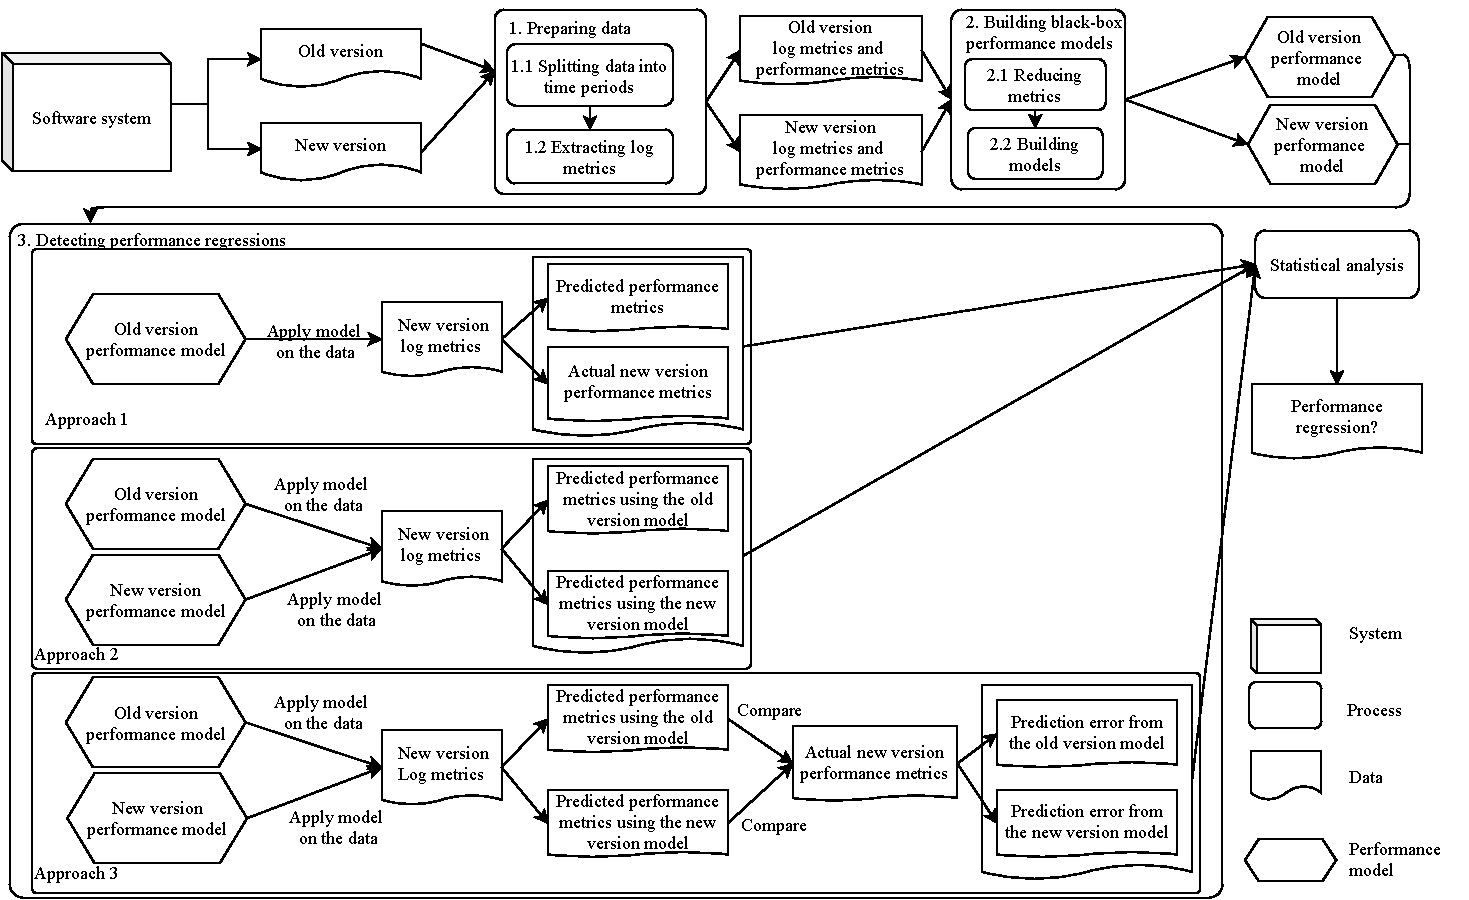
\includegraphics[width=\textwidth]{tex/figure/overview.pdf}
%   \vspace{-0.8cm}
  \caption{An overview of our studied approaches of detecting performance regressions.}
  %https://drive.google.com/file/d/1A1tein8v9yfW_aKvJKvpY4Radwsw--U6/view?usp=sharing
  
  \label{fig:overview}
%   \vspace{-0.35cm}
\end{figure*}



\subsection{Building black-box performance models}
\label{sec:buildmodel}
In this step, we build black-box models based on the log metrics and performance metrics that are collected and calculated from the data that is generated during system runtime under varied workloads. 

\subsubsection{Reducing metrics}
%The number of frequency of log events that do not change overtime are often due to the periodical events and the constant appearance of such events may not provide information about varied system workloads.
The frequency of some log events (e.g., periodical events) may not change over time.
The constant appearance of such events may not provide information about the changes of system workloads.
Therefore, after we calculate the log metrics of each log event, we reduce log metrics by removing redundant log metrics or log metrics with constant values in both previous and current versions. We first remove log metrics that have zero variance in both versions of the performance tests. 

Different log events may always appear at the same time, e.g., user logging in and checking user's privilege, and provide repetitive information for the workloads. To avoid the bias from such repetitive information, we then perform correlation analysis and redundancy analysis on each log metrics. We use Pearson's correlation coefficient~\citep{benesty2009pearson} among all log metrics. If a pair of log metrics has a correlation higher than $0.7$, we remove the metric from the two metrics. We repeat such process until there exists no correlation higher than $0.7$. The redundancy analysis would consider a log metrics redundant if it can be predicted from a combination of other log metrics. We use each log metrics as a dependent variable and use the rest of log metrics as independent variables to build a regression model. We calculate the $R^2$ of each model. If the $R^2$ is larger than a threshold (e.g., 0.9), the current dependent variable (i.e., the log metrics) is considered redundant. We then remove the log metric with the highest $R^2$ and repeat the process until no log metrics can be predicted with $R^2$ higher than the threshold. 

We only apply this step when using traditional statistical models or machine learning models (like linear regression or random forest), while if a deep neural network (like convolutional neural network or recurrent neural network) is adopted to build the black-box performance models, we skip this step.


\subsubsection{Building models}
We build models that capture the relationship between a certain workload that is represented by the logs and the system performance. In particular, the independent variables are the log metrics from the last step and the dependent variable is the target performance metric (e.g., CPU usage). One may choose different types of statistical, machine learning or deep learning models, as our approach is agnostic to the choice of models. However, the results of using different types of models may vary (cf. RQ1). 


%\subsubsection{Building models using data from the current version}
%In this step, we build new models that are built with new version data,  but that is not fair because the new data we are predicting is in our new data model. The model is biased toward the new data. So we take care of one new piece of data at a time,  We remove this row out of the new data. Then we use the rest of the new data to build the new model.

\subsection{Detecting performance regressions} \label{sec:comparions-approaches}

The goal of building the performance models is to detect performance regressions. Therefore, in this step, we use the black-box performance models that are built from an old version of the system to predict the expected system performance of a new version. Then, we use statistical analysis to determine whether there exists performance deviance based on prediction errors of the models.

Intuitively, one may use the model that is built from the old version of the system to predict the performance metrics from running the new version of the system. By measuring the prediction error, one may be able to determine whether there exists performance deviance~\citep{DBLP:conf/osdi/CohenCGKS04,DBLP:conf/wosp/NguyenAJHNF12}. However, such a naive approach may be biased by the choice of thresholds that are used to determine whether there is performance deviance. For example, a well-built performance model may only have less than 5\% average prediction error; while another less fit performance model may have 15\% average prediction error. In these cases, it is challenging to determine whether an average prediction error of 10\% on the new version of the system should be considered as a performance regression. Therefore, statistical analyses are used to detect performance regressions in a systematic manner~\citep{DBLP:conf/icst/GaoJBL16,DBLP:conf/wosp/ShangHNF15,Foo:2015:ICS:2819009.2819034}. 

In particular, we leverage three approaches to detect performance regressions: \emph{Approach 1}) by comparing the predicted performance metrics (using the model built from the old version) and the actual performance metrics of the new version, \emph{Approach 2}) by comparing the predicted performance metrics of the new version using the model built from the old version and the model built from the new version, and \emph{Approach 3}) by comparing the prediction errors of the performance metrics on the new version using the model built from the old version and the model built from the new version. We describe each approach in detail in the rest of this subsection.
%\subsubsection*{Approach 1: comparing the predicted value and the actual value of performance metrics from the new version}\hfill
%\vspace{-0.35cm}
%\subsubsection*{Approach 1: comparing the predicted performance metrics (using the model built form the old version) and the actual performance metrics of the new version}\hfill
\noindent\textbf{Approach 1: }\emph{comparing the predicted performance metrics (using the model built form the old version) and the actual performance metrics of the new version.} %\hfill
The most intuitive way of detecting performance regression is to compare the predicted value and the actual value of performance metrics. Since the model is built from the old version of the system, if there exists a large error between the predicted value and the actual value of the performance metrics from the new version of the system, we may consider the existence of performance regressions. In particular, we use the data from the old version of the system, i.e., $Data_{old}$ to build a black-box performance model $Model_{old}$ (cf. Section~\ref{sec:buildmodel}). Afterwards, we apply the model $Model_{old}$ on the data from the new version of the system, i.e., $Data_{new}$. Then we compare the predicted and the actual values of the performance metrics.


%\subsubsection*{Approach 2: comparing the predicted performance metrics of the new version using the model built from the old version and the model built from the new version}\hfill
\noindent\textbf{Approach 2: }\emph{comparing the predicted performance metrics of the new version using the model built from the old version and the model built from the new version.} %\hfill
Since our approach aims to be applied on varying workloads, the performance regression may only impact a small number of time periods, while the source code with performance regressions may not be executed in other time periods. Therefore, only the time periods that are impacted by the performance regressions may contain large prediction errors. To address such an issue, we also built a performance model $Model_{new}$ using the data from the new version of the system ($Data_{new}$). 
This way, $Model_{new}$ is built using the data with potential performance regressions. 
Afterwards, we use $Model_{old}$ and $Model_{new}$ to predict the performance metrics in $Data_{new}$. 

Since $Model_{new}$ is built from $Data_{new}$, there exist a bias when applying $Model_{new}$ on $Data_{new}$. To avoid the bias, instead of building one $Model_{new}$, we build $n$ models, where $n$ is the number of data points that exist in $Data_{new}$. In particular, for each data point in $Data_{new}$, we build a performance model $Model_{new}^n$ by excluding that data point and apply the model $Model_{new}^n$ on the excluded data point. Therefore, for $n$ data points from $Data_{new}$, we end up having $n$ models and $n$ predicted values. 

Finally, we compare the predicted values using $Model_{old}$ on $Data_{new}$, and the predicted values by applying each $Model_{new}^n$ on each of the $n$ data points in $Data_{new}$.


%\subsubsection*{Approach 3: comparing the prediction errors on the new version using the model built from the old version and the model built from the new version}\hfill
\noindent\textbf{Approach 3: }\emph{comparing the prediction errors on the new version using the model built from the old version and the model built from the new version.} %\hfill
The final approach of detecting performance regression is similar to the previous one (Approach 2), where instead of directly comparing the predicted performance metrics, we compare the distribution of the prediction errors by applying $Model_{old}$ on $Data_{new}$, and the predicted errors by applying each $Model_{new}^n$ on each of the $n$ data points in $Data_{new}$. The intuition is that when $Model_{old}$ has a larger prediction error than $Model_{new}$, it may be an indication of performance deviance between the two versions. We note that this approach would only be able to determine whether there exists performance deviance, which may actually be improvement instead of regression. 

%In order to address such a challenge, one may considering comparing the prediction error from applying the performance model on the old version itself and on the new version. However, this may have contain bias since the performance model itself is built from the old version of the system. Applying the model on the old version would potentially false show lower prediction errors. \heng{We may consider reducing some text in this paragraph.}

%In order to address the above challenges, in this step, we first calculate the prediction errors, i.e., $P_{new->old}$ \heng{Would it be the other way around, $P_{old->new}$?}, by applying the performance model that is built from the old version of the system on the data from the new version of the system. Afterwards, we calculate the prediction errors, i.e., $P_{new->new}$, by applying the performance model that is built from the new version of the system on the data from the new version of the system. To avoid the bias of calculating $P_{new->new}$ using the model built and tested on the same data, instead of building one model using the data from the new version of the system, we build $n$ models, where $n$ is the number of data points that exist in the data from the new version of the system. In particular, for each data point in the data from the new version of the system, we build a performance model by excluding that data point and calculate the prediction error by applying the model on the excluded data point. Therefore, for $n$ data points from the new version of the system, we end up having $n$ models and $n$ prediction errors, each calculated by one data point. Therefore, $P_{new->new}$ would contain $n$ prediction error values, which can be compared against the prediction errors in $P_{new->old}$ to identify performance deviance.


%\subsubsection*{\underline{Statistical analysis}}\hfill
\noindent\textbf{Statistical analysis.}
All the three approaches generate two distributions of either actual/predicted performance metric values, or prediction errors. With two distributions of data at hand, we compare the two distributions similar to previous studies~\citep{Chen:2016:CHD:2950290.2950303} using statistical tests and effect sizes. In particular, we use the Mann-Whitney U test since it is non-parametric and it does not assume a normal distribution of the compared data. we run the test at the 5\% level of significance, i.e., if the P-value of the test is not greater than 0.05, we would reject the \emph{null hypothesis} in favour of the alternative hypothesis, i.e., there exists a statistically significant difference between the two distributions. In order to study the magnitude of the difference without being biased by the size of the data, we further adopt the effect size  as a complement
of the statistical significance test. Considering the non-normality of our data points, we
utilize \emph{Cliff's Delta}~\citep{cliff1996ordinal} using the
thresholds provided in prior research~\citep{romano2006appropriate}.


